\documentclass[]{article}
\usepackage[utf8]{inputenc}
\usepackage[T1]{fontenc}
\usepackage[dvipsnames]{xcolor}
\usepackage{lmodern}
\usepackage{amssymb,amsmath}
\usepackage{textgreek}
\usepackage{ifxetex,ifluatex}
\usepackage{todonotes}
\usepackage{xifthen}
\usepackage{soul}
\usepackage[american]{babel}
\usepackage[ruled]{algorithm2e}

\usepackage[backend=biber,style=apa]{biblatex}
\addbibresource{DreamReplay.bib}
\DeclareLanguageMapping{american}{american-apa}
\sethlcolor{Apricot}
\newcommand\bla[1]{\ifthenelse{\isempty{#1}}{\hl{**~bla~bla~**}}{\hl{**~#1~**}}}

% use upquote if available, for straight quotes in verbatim environments
\IfFileExists{upquote.sty}{\usepackage{upquote}}{}
\ifnum 0\ifxetex 1\fi\ifluatex 1\fi=0 % if pdftex
  \usepackage[utf8]{inputenc}
\else % if luatex or xelatex
  \ifxetex
    \usepackage{mathspec}
    \usepackage{xltxtra,xunicode}
  \else
    \usepackage{fontspec}
  \fi
  \defaultfontfeatures{Mapping=tex-text,Scale=MatchLowercase}
  \newcommand{\euro}{€}
\fi
% use microtype if available
\IfFileExists{microtype.sty}{\usepackage{microtype}}{}
\ifxetex
  \usepackage[setpagesize=false, % page size defined by xetex
              unicode=false, % unicode breaks when used with xetex
              xetex]{hyperref}
\else
  \usepackage[unicode=true]{hyperref}
\fi
\usepackage[all]{hypcap} % ref link to the top of the figure

\usepackage{csquotes} % Dependency for APA


\hypersetup{breaklinks=true,
            pdfauthor={Paul Ecoffet},
            pdftitle={Rapport de stage},
            colorlinks=true,
            citecolor=blue,
            urlcolor=blue,
            linkcolor=magenta,
            pdfborder={0 0 0}}
\urlstyle{same}  % don't use monospace font for urls
\setlength{\parindent}{0pt}
\setlength{\parskip}{6pt plus 2pt minus 1pt}
\setlength{\emergencystretch}{3em}  % prevent overfull lines
\setcounter{secnumdepth}{0}

\title{Can the replayed sequences during sleep can be modelised by a reinforcement learning algorithm? -- Rapport de stage}
\author{Paul Ecoffet}
\date{15 avril 2016}


\begin{document}
\maketitle

\begin{abstract}
% Première phrase trop proche de l'abstract de Gupta.
On the neurobiology side, replays of behavioral sequences have been observed in the hippocampus during sharp wave ripples complexes and is thought to be a mechanism involed in memory consolidation and learning. On the computer science side, some reinforcement learning algorithms also use replays of behavioral sequences to improve the learning speed. One can ask if this algorithms behave in the same way that hippocampus replays of sequences, and if these algorithms can model the replay mechanisms observed in the hippocampus. For instance, can those algorithms explain why certain sequences are replayed instead of others? We'll show that that \bla{we'll see}.
\end{abstract}

{
\hypersetup{linkcolor=black}
\setcounter{tocdepth}{3}
%\tableofcontents
}
\section{Introduction}\label{introduction}

\subsection{Reinforcement learning}\label{reinforcement-learning}

Reinforcement Learning is a kind of learning mechanism where an agent tries to maximise a reward by doing some specific action in an environment \parencite{sutton_reinforcement_1998}. The environment is defined by set of \emph{states} (noted \(\mathcal{S}\)) in which the agent can be. In each state, the agent can do an \emph{action} from its \emph{action set} (noted \(\mathcal{A}\)). When doing a specific action \(a\) in a specific state \(s\), the agent receives a \emph{reward} (noted \(r\)) and go in a new state \(s'\in \mathcal{S}\). The reward is a number which can be positive or negative. The goal of the agent is to maximise the amount of reward it receives over time. The agent must do the best action in a given state to get the most reward in the long run. This mean that it might be worthful to go in a state which gives no reward if it can lead to new states that give a high reward. The table which links each state to an action is called a \emph{policy}. Reinforcement learning are methods to find the best policies in a given environment.

This kind of environment and task is called a \emph{Markov Reward Process}. This process can be used to model a wide variety of situation such as maze solving tasks or workload management \parencite{sutton_reinforcement_1998,vanseijen_deeper_2015}.

For instance, we can model experiences on rats who does maze solving task with markovian reward process. For instance, if we model a tree maze, each state is a node of the tree, the action of the rat is to take a edge. When it does so, he goes to another node (a new state), and receive the amount of food pellets in this node. Figure~\ref{fig:mdp_tree} shows an exemple of such maze. In this model, the goal of the rat is to eat as much food pellets as possible. The agent must maximise its amount of reward over time.

\begin{figure}[htpb]
  {\centering
  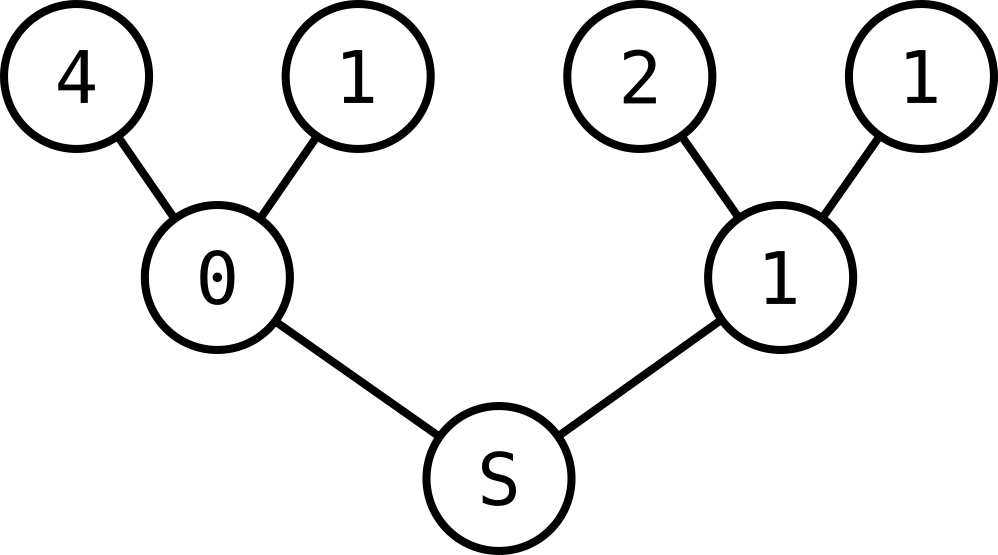
\includegraphics[width=0.4\linewidth]{images/mdp_tree.png}
  \caption{Exemple of an environment with states and rewards\label{fig:mdp_tree}}}
  \small
  Each number is the reward associated with the state. The goal of the agent is to maximise the amount of reward it gets in an episode. Therefore, he has to choose the action ``go left'' to get the 0, then choose ``go left'' again to get the 4.
\end{figure}

If the agent knows his environment perfectly, it is possible to find the best policy to maximise the amount of reward the agent gets in the long run analytically.

To know if it is ``interesting'' to go into a state \(s\), the agent can compute the \emph{value} \(V_\pi\) of it. The value of a state is the expected reward the agent will receive if he is in this state plus the future rewards it can get from future states according to its policy \(\pi\). Rewards from future states are discounted by a coefficient \(\gamma\).

\begin{equation}
  V_\pi(s) = r_{s, a} + \gamma \sum_{a\in\mathcal{A}} \pi(s,a)\sum_{s'\in\mathcal{S}} P(s'|s, a) V(s')
\end{equation}

With complete knowledge of the rewards \(r\), the transition table of state according to an action (ie. the fact that I will be in \(s'\) if I do action \(a\) while in \(s\)), the value of every state can be computed according to the agent's policy. It is then possible to compute the best policy possible analytically or iteratively with Expectation-Maximisation (EM) algorithm \parencite{sutton_reinforcement_1998}.

When the environment is not known by the agent, the value function cannot be computed and it must be approximated. The agent explore the environment and observe for each state the reward it gets, the next state it will be according to its action and update a value function approximation \(\tilde{V}_\pi\). Different methods such as Monte Carlo or Temporal Difference (TD) provide way to approximate \(V\). Then, the policy can be updated with an EM algorithm on \(\tilde{V}_\pi\) or use another policy improvement method. \cite{,,}

\subsection{Temporal Difference algorithm}

Temporal difference (TD) algorithms are methods that do not require a perfect knowledge of the environment. The TD(0) algorithm (Algorithm~\ref{alg:td0}) is the most basic TD learning algorithm. TD(0) algorithm computes an approximation of \(\tilde{V}_\pi\) after each action of the agent, using the equation~\ref{td_approx_v}.

\begin{equation}
  \hat{V}_\pi(s) = r + \gamma \tilde{V}_\pi(s')
  \label{td_approx_v}
\end{equation}

The \(\hat{V}_\pi(s)\) which is computed takes only into account the next state \(s'\) the agent happens to be in after taking its action, and not all the possible outcomes as \(V_\pi(s)\) does. \(\tilde{V}_\pi(s)\) is updated slightly toward \(\hat{V}_\pi(s)\) so that in the long run, \(\tilde{V}_\pi(s)\) takes into account every outcome \(r\) and \(s'\) possible, according to their probability of occurence. To do so, a \emph{learning rate} parameter \(\alpha \in ]0, 1[\) is set, and \(\tilde{V}_\pi(s)\) is updated with the formula in equation~\ref{v_tilde_learning_rate}.

\begin{equation}
\tilde{V}_\pi(s) = \tilde{V}_\pi(s) + \alpha (\hat{V}_\pi(s) - \tilde{V}_\pi(s))
\label{v_tilde_learning_rate}
\end{equation}

TD learning and reinforcement learning is fully covered in \textcite{sutton_reinforcement_1998}.

\begin{algorithm}[htbp]
  \DontPrintSemicolon
  \SetAlgoNoLine
  \KwIn{current \(\tilde{V}\) (usually \(\vec{0}\)), first state \(s\), policy \(\pi\), learning rate \(\alpha\), discount factor \(\gamma\)}
  \KwOut{Updated \(\tilde{V}\)}
  \While{s \textbf{is not} end}{
    \(a \gets\) action according to \(\pi\) for \(s\)\;
    Do \(a\), observe the reward \(r\) and the new state \(s'\)\;
    \(\delta \gets r + \gamma \tilde{V}(s') - \tilde{V}(s)\)\;
    \(\tilde{V}(s) \gets \tilde{V}(s) + \alpha \delta\)\;
    \(s \gets s'\)\;
  }
  \caption{Canonical TD(0)  \label{alg:td0}}

\end{algorithm}

It is interesting to note that the Temporal Difference \(\delta\), which correspond to the error between the expected value of a state and the actual value observed (\(\hat{V}_\pi(s) - \tilde{V}_\pi(s)\)), has been correlated with the dopaminergic response of neurons by \textcite{hollerman_dopamine_1998}.


\subsection{Learning by replay}\label{learning-by-replay}

\subsubsection{In reinforcement learning}
\label{sub:In reinforcement learning}

Reinforcement learning methods based on TD(0) like Sarsa or Q-Learning converge slowly and need a lot of samples to be efficient. These algorithms use the sample once to improve their solution, then discard it \parencite{adam_experience_2012}.

To improve the efficiency of reinforcement learning methods, one solution is to replay past experiences. \textcite{vanseijen_deeper_2015} offers a good analysis about learning by replay. The goal of replay is to use the maximum of information an experience offers. Each sample is used several times using the current knowledge of the agent, improving the solution several times. Compared to TD(0), replay techniques give a better convergence to the optimal solution with the same number of experiences. Reinforcement learning methods using replay are more expensive than TD(\textlambda) both in memory and in computations, though the memory and computational power needed can be reduced a lot as \textcite{vanseijen_deeper_2015} shows.

\textcite{vanseijen_deeper_2015} give a canonical TD(0) algorithm with replay. This algorithm puts in a list \(\mathcal{M}\) all the states, reward and transition the agent have observed at each step. After each action, the algorithm use the new value function estimation it has to replay previous states to compute from the beginning of the experience a new value function estimation given these previous states (in \(\mathcal{M}\)) and the current knowledge it has (\(\tilde{V}_\pi\)).

Note that starting from now, I will no longer use \(\pi\) as an indice for the value function to thow that the value function depends on the policy \(\pi\), but I will put as indice the time step at which the estimation has been done. \(\tilde{V}_4\) correspond to the estimation of the value function the algorithm gets after its forth action (of course, according to a policy \(\pi\)). It is also understated that \(\tilde{V}_{t+1} = \tilde{V}_{t}\) for every state except from the one for whom the function has been updated.

The example of computation of \(\tilde{V}_\pi\) using replay proposed by \textcite{vanseijen_deeper_2015} is given in equations~\ref{ex_eq_td0}~and~\ref{ex_eq_td0_replay}. Equation~\ref{ex_eq_td0} shows the updates of a canonical TD(0) algorithm, as in algorithm~\ref{alg:td0}.

\begin{equation}
  \begin{aligned}
    \tilde{V}_{1}(s_0) &\gets \tilde{V}_0(s_0) + \alpha (r_1 + \gamma \tilde{V}_0(s_1) - \tilde{V}_0(s_0))\\
    \tilde{V}_{2}(s_1) &\gets \tilde{V}_1(s_1) + \alpha (r_2 + \gamma \tilde{V}_1(s_2) - \tilde{V}_1(s_1))\\
    \tilde{V}_{3}(s_2) &\gets \tilde{V}_2(s_2) + \alpha (r_3 + \gamma \tilde{V}_2(s_3) - \tilde{V}_2(s_2))\\
  \end{aligned}
  \label{ex_eq_td0}
\end{equation}

The idea of replay is to use the knowledge got after some time. For instance, let \(\tilde{V}_* = \tilde{V}_3\). Then, it is possible to compute a new estimate of the value function from scratch using this knowledge and past experiences:

\begin{equation}
  \begin{aligned}
    \tilde{V}_{1}'(s_0) &\gets \tilde{V}_0(s_0) + \alpha (r_1 + \gamma \tilde{V}_*(s_1) - \tilde{V}_0(s_0))\\
    \tilde{V}_{2}'(s_1) &\gets \tilde{V}_1'(s_1) + \alpha (r_2 + \gamma \tilde{V}_*(s_2) - \tilde{V}_1'(s_1))\\
    \tilde{V}_3'(s_2) &\gets \tilde{V}_2'(s_2) + \alpha (r_3 + \gamma \tilde{V}_*(s_3) - \tilde{V}_2'(s_2))\\
  \end{aligned}
  \label{ex_eq_td0_replay}
\end{equation}

\(\tilde{V}'\) is reasonably more accurate that \(\tilde{V}\), as stated by \textcite{vanseijen_deeper_2015}. Using the same method, \(\tilde{V}''\) can be computed using the same method and with \(\tilde{V}_* = \tilde{V}'_3\) and so on, depending of the computational budget of the algorithm. The algorithm~\ref{alg:td0_replay} can therefore be constructed \parencite{vanseijen_deeper_2015}.

\begin{algorithm}[htbp]
  \DontPrintSemicolon
  \SetAlgoNoLine
  \KwIn{\(\tilde{V}_{init}\) (usually \(\vec{0}\)), first state \(s\), policy \(\pi\), learning rate \(\alpha\), discount factor \(\gamma\), computational budget \(k\)}
  \KwOut{Updated \(\tilde{V}\)}
  \(\tilde{V} \gets \tilde{V}_{init}\)\;
  \(\mathcal{M} \gets \emptyset\) \tcp{The list of observed samples}
  \While{s \textbf{is not} end}{
    \(a \gets\) action according to \(\pi\) for \(s\)\;
    Do \(a\), observe the reward \(r\) and the new state \(s'\)\;
    append \((s, r, s')\) to \(\mathcal{M}\)\;
    \For{\(i \gets 1\) to \(k\)}{
      \(\tilde{V}_* \gets \tilde{V}\)\;
      \(\tilde{V} \gets \tilde{V}_{init}\)\;
      \ForEach{\((s, r, s') \in \mathcal{M}\) (from oldest to newest)}{
        \(\delta \gets r + \gamma \tilde{V}_*(s') - \tilde{V}(s)\)\;
        \(\tilde{V}(s) \gets \tilde{V}(s) + \alpha \delta\)\;
      }
    }
    \(s \gets s'\)\;
  }
  \caption{TD(0) with Replay \label{alg:td0_replay}}

\end{algorithm}

\subsubsection{Planning and replay?}
\label{subs:Planning and replay}

RL algorithms with planning use a model of their environment to infer the value  of a behaviour without actually doing it. The model is commonly a transition table between the possible states in the environment according to the action done by the agent. For exemple, if the agent has to solve a maze and has access to a transition table, then it can look up the table and know that if he is in the case \((3, 5)\) and it does the action ``go to the east'', it will be in \((4, 5)\), without actually doing the action.

The model can be either directly accessible (given by the developer) or inferred by the agent. When the model is inferred, the agent builds explicitly the transition table according to the experiences he has in its environment. In this document, we will mainly talk about the Dyna algorithms. Dyna is a class of RL algorithms where the model is inferred by the agent. There is two phase during an iteration of Dyna. The first phase is when the agent interacts with its environment: it observes its state and reward, do an action according to its policy and go to the next state. It also updates its model of the environment according to this new experience. The second part is the \emph{planning} phase. During the planning phase, the agent improves its value function estimation with simulations according to its model: The agent generates a sample state, an experience, according to some rules (a probability distribution) and uses its model to compute the value of this sample thanks its model. Then, it updates its solution according to this simulation \parencite{sutton_dyna-style_2012}.
Algorithm~\ref{alg:canonical_dyna} from \textcite{sutton_dyna-style_2012} is the canonical form of a Dyna algorithm. In this algorithm and next algorithms, \(F\) and \(b\) represent the model of the environment built by the agent. \(F\) is a transition matrix. If \(\phi\) is the current feature vector of the state the agent is, then \(\phi' = F\phi\) is the estimated feature vector of the next state the agent will be according to its policy \(\pi\). \(b\) is the expected reward per feature activation vector. For instance, if all the features observed by the agent are at \(0\) except from the \(i\)-th feature is at \(2\) and \(b_i = 0.25\), then the expected reward for this state according to the agent's model is \(\hat{r} = 0.5\).The expected reward from a feature vector according to the model of the agent is given by equation~\ref{expected_reward}.

\begin{equation}
\hat{r} = b^\top \phi \label{expected_reward}
\end{equation}

\begin{algorithm}[htbp]
  \DontPrintSemicolon
  \SetAlgoNoLine
  \KwIn{\(\theta_{init}\) (usually \(\vec{0}\)), first features vector \(\phi\), policy \(\pi\), learning rate \(\alpha\), discount factor \(\gamma\), computational budget \(k\)}
  \KwOut{Updated \(\theta\)}
  \(\theta \gets \theta_{init}\)\;
  \While{\textbf{not} end}{
    \(a \gets\) action according to \(\pi\) for \(\phi\)\;
    Do \(a\), observe the reward \(r\) and the new state \(\phi'\)\;
    \(\theta \gets \theta +
        \alpha(r + \gamma\theta^\top\phi' - \theta^\top\phi)\phi\)\;
    \(F \gets F + \alpha(\phi' - F\phi)\phi^\top\)\;
    \(b \gets b + \alpha(r - b^\top\phi)\phi\)\;
    \(mem \gets \phi'\)\;
    \For{\(i \gets 1\) to \(k\)}{
      Generate a sample \(\phi\) from distribution \(\mu\)\;
      \(\phi' \gets F\phi\)\;
      \(r \gets b^\top\phi\)\;
      \(\delta \gets r + \gamma \theta^\top\phi' - \theta^\top(\phi)\)\;
      \(\theta \gets \theta + \alpha \delta\)\;
    }
    \(\phi \gets mem\)\;
  }
  \caption{Canonical Linear Dyna \label{alg:canonical_dyna}}
\end{algorithm}


It is interesting to note that the distribution used to draw samples has no influence on whether the solution will converge or not as long as it covers all the possible features, but has an influence on the speed of convergence. Therefore, choosing a good distribution can greatly improve the performance of Dyna. \textcite{sutton_dyna-style_2012} shows that choosing only already explored samples can have a good impact on convergence speed. Therefore, even if \textcite{sutton_dyna-style_2012} do not explicitly say it, the planning phase is then a \emph{replay} phase. In their paper, they present two algorithms which use replays: Linear  Dyna  with  PWMA  prioritized sweeping (LD-PWMA) and Linear Dyna with MG prioritized sweeping (LD-MG). Both these algorithm store all the features the agent encounters in a queue. The features are then drawn from this queue during the planning/replay phase. The idea of prioritized sweeping is to draw the samples in a specific order according to a criterion which will speed up the convergence. PWMA and MG use both a function of the difference between the expected value of the state and its actual value, the value \(\delta\), as the criterion to sort the samples. \textcite{sutton_dyna-style_2012} show that Linear Dyna with MG prioritized sweeping (LD-MG) out performs several classic RL algorithms and PWMA-LD in speed of convergence for classical RL problems.

Algorithm~\ref{alg:mg_dyna} is the pseudo code implementation of Linear Dyna with MG prioritized sweeping policy evaluation.

\begin{algorithm}[htbp]
  \DontPrintSemicolon
  \SetAlgoNoLine
  \KwIn{\(\theta_{init}\) (usually \(\vec{0}\)), first feature vector \(\phi\), policy \(\pi\), learning rate \(\alpha\), discount factor \(\gamma\), computational budget \(k\)}
  \KwOut{Updated \(\tilde{\theta}\)}
  \(\theta \gets \theta_{init}\)\;
  Init PQueue\;
  \While{\textbf{not} end}{
    \(a \gets\) action according to \(\pi\) for \(\phi\)\;
    Do \(a\), observe the reward \(r\) and the new state \(\phi'\)\;
    \(\delta \gets r + \gamma \theta^\top\phi' - \theta^\top\phi\)\;
    \(\theta \gets \theta +
        \alpha\delta\)\;
    \(F \gets F + \alpha(\phi' - F\phi)\phi^\top\)\;
    \(b \gets b + \alpha(r - b^\top\phi)\phi\)\;
    \ForAll{\(i\) such as \(\phi(i) \neq 0\)}{
      Put \(i\) on the PQueue with priority \(|\delta\phi(i)|\)\;
    }
    counter \(\gets 0\)\;
    \While{PQueue \textbf{is not} empty \textbf{and} counter \(\leq k\)}{
      \(\phi' \gets F\phi\)\;
      \(r \gets b^\top\phi\)\;
      \(\delta \gets r + \gamma \tilde{V}_*(s') - \tilde{V}(s)\)\;
      \(\tilde{V}(s) \gets \tilde{V}(s) + \alpha \delta\)\;
    }
    \(phi \gets mem\)\;
  }
  \caption{Linear Dyna with MG prioritized sweeping \label{alg:mg_dyna}}

\end{algorithm}

\textcite{vanseijen_deeper_2015} highlights even more the strong similarity between RL methods using replay and RL methods using planning. First of all, both of them can be considered as model-based algorithms. Indeed, planning methods using an inferred model use an integrated version of samples experienced over time, thus they are by definition model-based algorithms.
RL algorithms using experience replay do not store an explicit model, with transition tables and reward estimation. Yet, they store for each sample the state they were in, the reward they received and the next action they did. These data can be considered as a model. They implicitly contains an inferred model of the environnement. Transitions and rewards are available through all the samples the agent experienced and stored in memory \parencite{vanseijen_deeper_2015}. This is


In addition to that, \textcite{vanseijen_deeper_2015} shows a complete equivalence in the value function approximation at each iteration between a TD(0) inspired algorithm with replay and Linear Dyna, a model-based RL algorithm. Though Linear Dyna is a model based algorithm and thought as a ``looking ahead'' algorithm and the replay algorithm as a ``looking backward'' algorithm, they do the exact same calculation.
The Linear Dyna variation \textcite{vanseijen_deeper_2015} presents is a batch Linear Dyna. Each iteration of planning compute using an integrated version of all the states and transition experienced. One can ask if different variations of Linear Dyna can also be considered as learning by replay methods. For instance, \textcite{sutton_dyna-style_2012} reviewed different Linear Dyna algorithms which look at one possible state per planning iteration. They shows that using already experienced states and prioritizing about states where the difference between the estimated value and the real value was the greatest is an efficient strategy.

\subsubsection{In vivo}
\label{sub:In vivo}

\paragraph{Place cells}\label{place-cells}
Place cells are high level integrative neurons in the hippocampus. They have a specific receptive field called a place field. When the animal is in the receptive field of a place cell, the place cell spikes. It is on these cells that the replay of behavioral sequences is observed during sleep.

\paragraph{Replay}
Replays of sequences have been observed in the rat hippocampus after navigation tasks \parencite{wilson_reactivation_1994, skaggs_replay_1996, davidson_hippocampal_2009, gupta_hippocampal_2010}. The place cells whose activations were highly correlated in time are also activated during sleep and respect the same correlation \parencite{wilson_reactivation_1994}. Replays of place cells activation sequences that occurs during the day can also be observed either forward \parencite{skaggs_replay_1996} or even backward \parencite{gupta_hippocampal_2010}. Coherent sequences that have never been done are also ``replayed'' by the rat \parencite{gupta_hippocampal_2010}. Though, those articles do not propose explantion about why these specific sequences were chosen or about the length of these sequences. \textcite{gupta_hippocampal_2010} shows that the recency of the experience is a wrong hypothesis but do not propose other explanation\todo{to check}. We will try to provide a criterion to explain why specific sequences are replayed and not others.



\begin{itemize}
\item Replay during sleep and during hesitation
\item Replay can be either forward or backward
\item Replay can also be action that has never be done? --> Planning somewhat?
\item Replay aren't necessary about the most recent event?
\item Is ``surprise'' a good crterion?
\end{itemize}

\subsection{Model navigation learning}\label{model-navigation-learning}

We can model place cells in a reinforcement learning algorithm by using a tiling of the environment (see Figure~\ref{tiling_schema}) as \textcite{	tamosiunaite_path-finding_2008} have done. Each feature of the feature vector (the state of the agent) represents the level of activation of a tile: a gaussian-like function of the distance of the agent from a kernel. For instance, the \(i^{th}\) feature of the feature vector will be the distance from the kernel \(k_i\) according to a gaussian function (see Figure~\ref{feature_schema}). The value of the \(i^{th}\) feature can be interpreted as the firing rate of a place-cell with a receptive field centered in \(k_i\).

\noindent\begin{figure}[htbp]
  \centering
  \begin{minipage}[t]{.5\linewidth}
    {\centering
    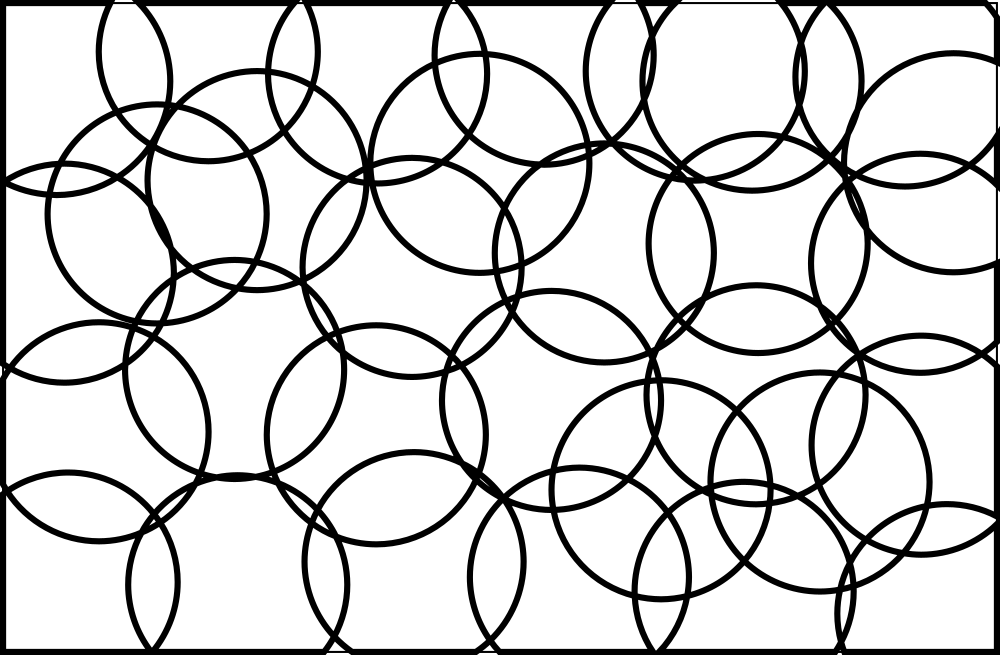
\includegraphics[width=0.9\linewidth]{images/schema_tiling.png}
    \caption{Tiling of an environment}\label{tiling_schema}
    \par}
    \small{Each disk can be thought as the receptive field of a place cell}
  \end{minipage}%
  \begin{minipage}[t]{.5\linewidth}
    \centering
    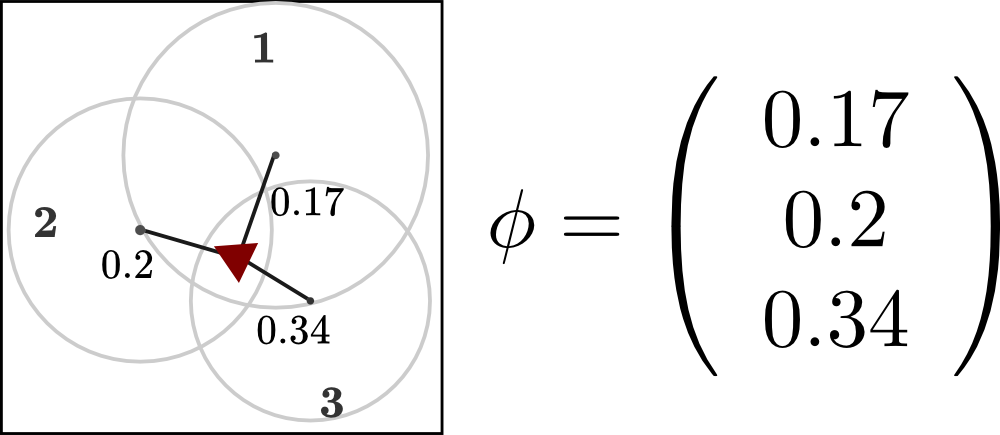
\includegraphics[width=0.9\linewidth]{images/feature_schema.png}
    \caption{Features representation}\label{feature_schema}
  \end{minipage}
\end{figure}



\subsection{What are the sequences that are replayed? How are they
selected?}\label{what-are-the-sequences-that-are-replayed-how-are-they-selected}

\textcite{gupta_hippocampal_2010} shows that the sequences that are replayed are not necessarly the most recent experiences. It shows also that the sequences that are replayed can be either forward or backward. In forward replays, the sequence is replayed in the same order as the sequence the rat has done. In backward replays, the sequence is done in the reverse order. What is the explanation for the selection of the sequence which is replayed, and its order? No criteria are proposed in \textcite{gupta_hippocampal_2010}. Yet, we can make interesting hypothesis knowing that \textcite{sutton_dyna-style_2012} suggests that there are very good samples to replay in a Dyna algorithm, and those sample are the sample where the difference between the expected value of a state and its real value is the greatest. It is consistant with \textcite{gupta_hippocampal_2010} which states that the most common replays are the one that leads to the reward or comes from the reward.

\section{Method}\label{method}
\begin{itemize}
  \item Pourquoi x place-cells?
  \item Pourquoi ce radius?
  \item Quel densité?
  \item Quel type d'activation?
\end{itemize}

I try to reproduce the results of \textcite{gupta_hippocampal_2010} and see if a Linear Dyna with prioritized sweeping as developped in \textcite{sutton_dyna-style_2012} can reproduce the results observed \emph{in vivo}. To do so, I have modelised the maze used by \textcite{gupta_hippocampal_2010}. The source code is available at \bla{github}. It is a continuous world.

\section{Results}\label{results}

\section{Conclusion}\label{conclusion}

\section{Limitations}\label{limitations}


\printbibliography{}

\end{document}
